\documentclass[]{article}

\usepackage[margin=1in]{geometry} \usepackage{url} \usepackage{parskip}
\usepackage{graphicx}
\usepackage{float}

\begin{document}

\title{Computer Visualization Report}
\author{Roy Portas}
\date{\today}
\maketitle

\section{Introduction}

Criminology is the study of causes, nature and prevention of criminal behaviour\cite{roufa_early_nodate}.
This study is important as it allows sociologists and psychologists to not only study the when and how crime occurs, but offers a way to predict crime trends in the future.

Crime is an evident part of our society and is an active topic during elections\cite{remeikis_queensland_2016}, even companies like IBM\cite{noauthor_ibm_2012} and Palantir\cite{palantir_technologies_law_nodate} 
are creating products to model, predict and prevent crimes before they happen.

As technology becomes more powerful, the cost of implementing systems capable of predicting crimes becomes more feasible.
However these systems are difficult to build, as it is almost impossible to predict the future.
Nevertheless companies have started building such systems.

Crime prediction systems generally consist of the following components:
\begin{itemize}
    \item Identify areas with frequent crime\cite{noauthor_ibm_2012}
    \item Match trends in national and regional crimes with local crimes
    \item Identify circumstances for the cause of crimes\cite{noauthor_ibm_2012}
\end{itemize}

\section{Aims}

This report aims to analyse and explore crime data for Queensland. A variety of techniques and datasets will be used to explore this problem, including:

\begin{itemize}
    \item Analyse reported offences by suburb, month and offence type to find relationships in crime over time.
    \item Analysis of geolocation data for crime locations and police districts
\end{itemize}

\section{Methods}

\section{Results}

\begin{figure}[H]
    \caption{Heatmap of crime over time}
    \centering
    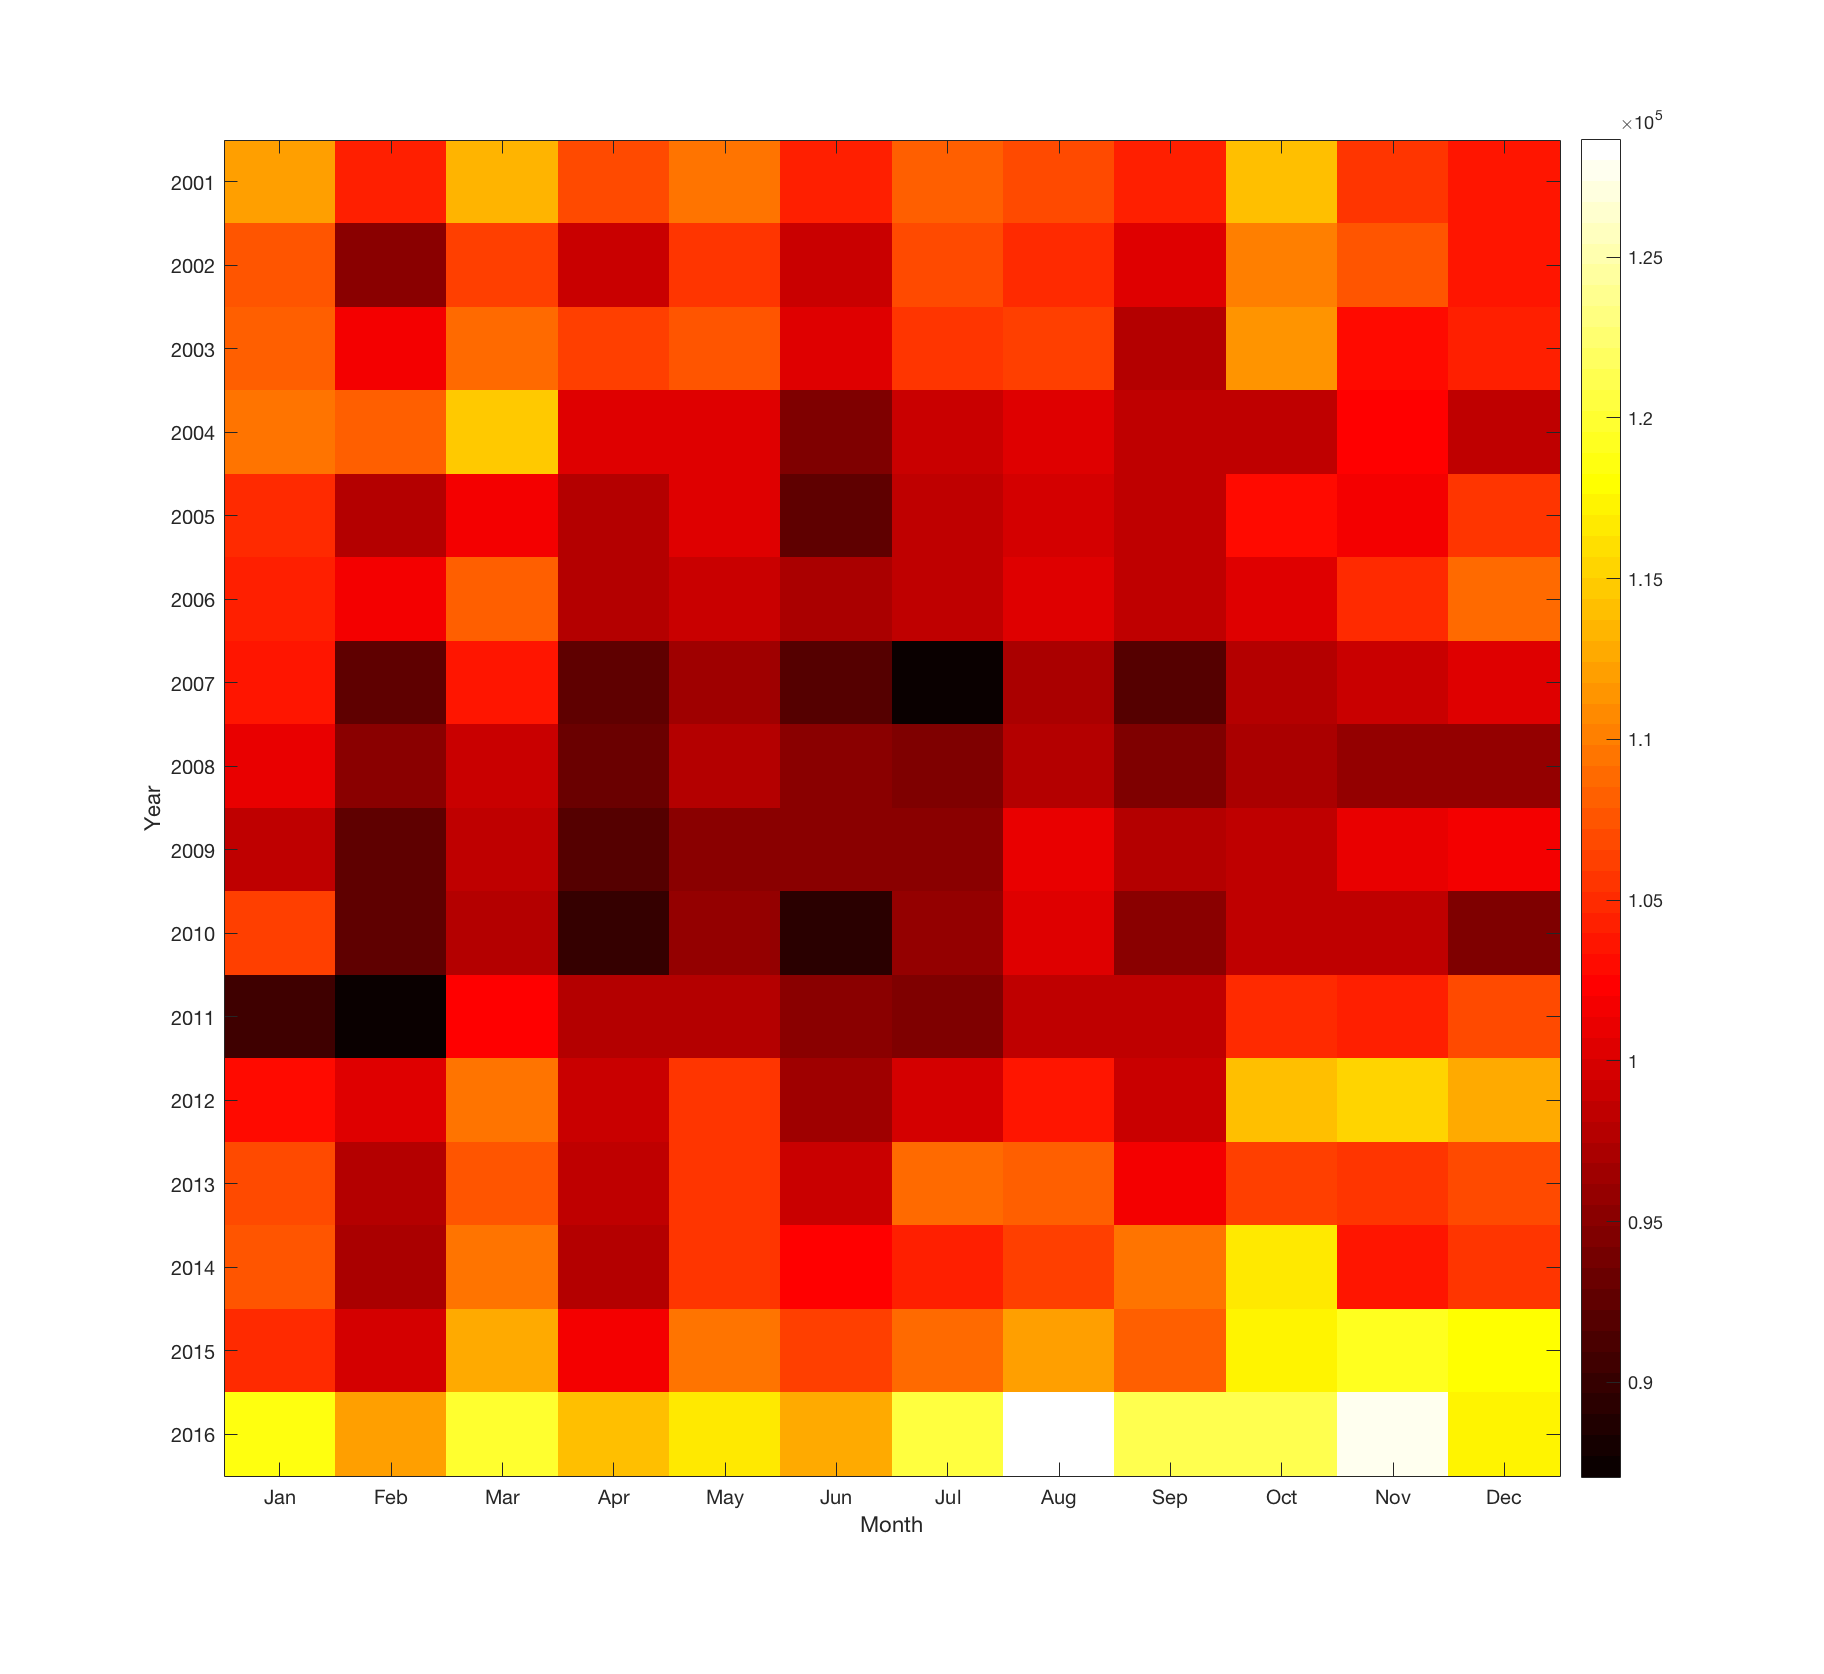
\includegraphics[width=\linewidth]{../images/crime_time_heatmap}
\end{figure}

A spike in crime was noticed during March 2004, this can also be seen in the other  charts below, historical records show that March was when the Brisbane City Council elections happened and Campbell Newman became the Lord Mayor of Brisbane\cite{noauthor_2004_2017}

\begin{figure}[H]
    \caption{Total offences over time}
    \centering
    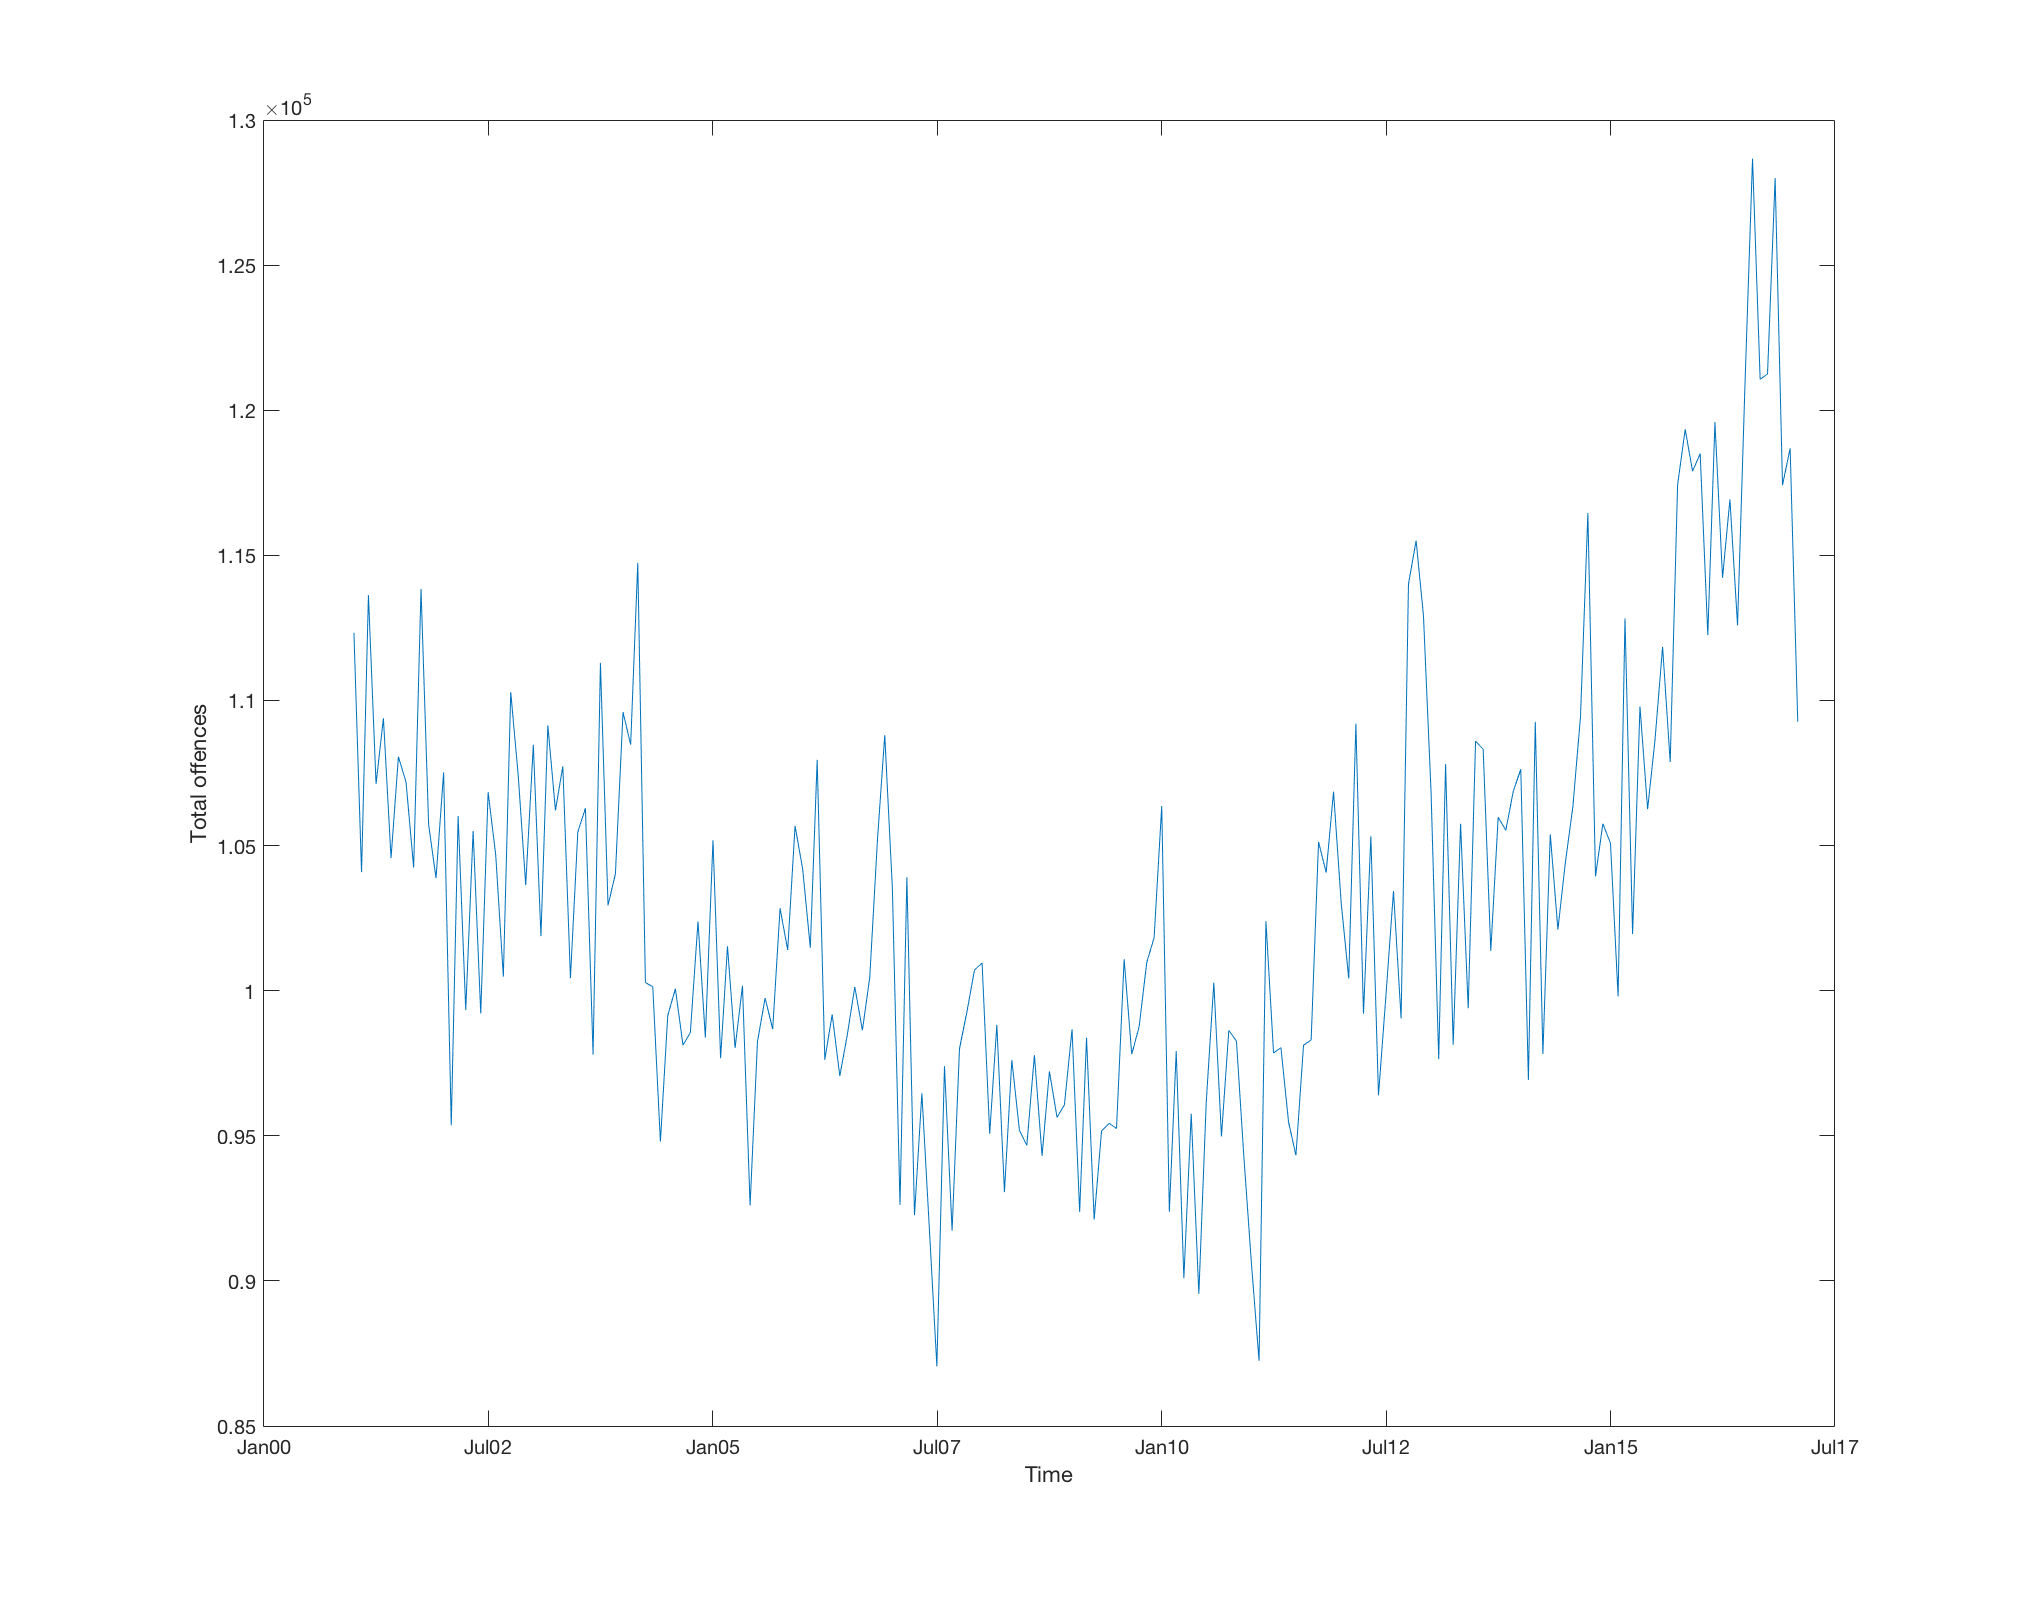
\includegraphics[width=\linewidth]{../images/crime_over_time}
\end{figure}

Sorting the crimes by the average number of offences determined that the most common crimes are

\begin{enumerate}
    \item Offences against property
    \item Other offences
    \item Other theft exculding unlawful entry
    \item Drug offences
    \item Unlawful entry
\end{enumerate}

These offences can be plotted against the months to see how they change over time.

\begin{figure}[H]
    \caption{Top offences over time}
    \centering
    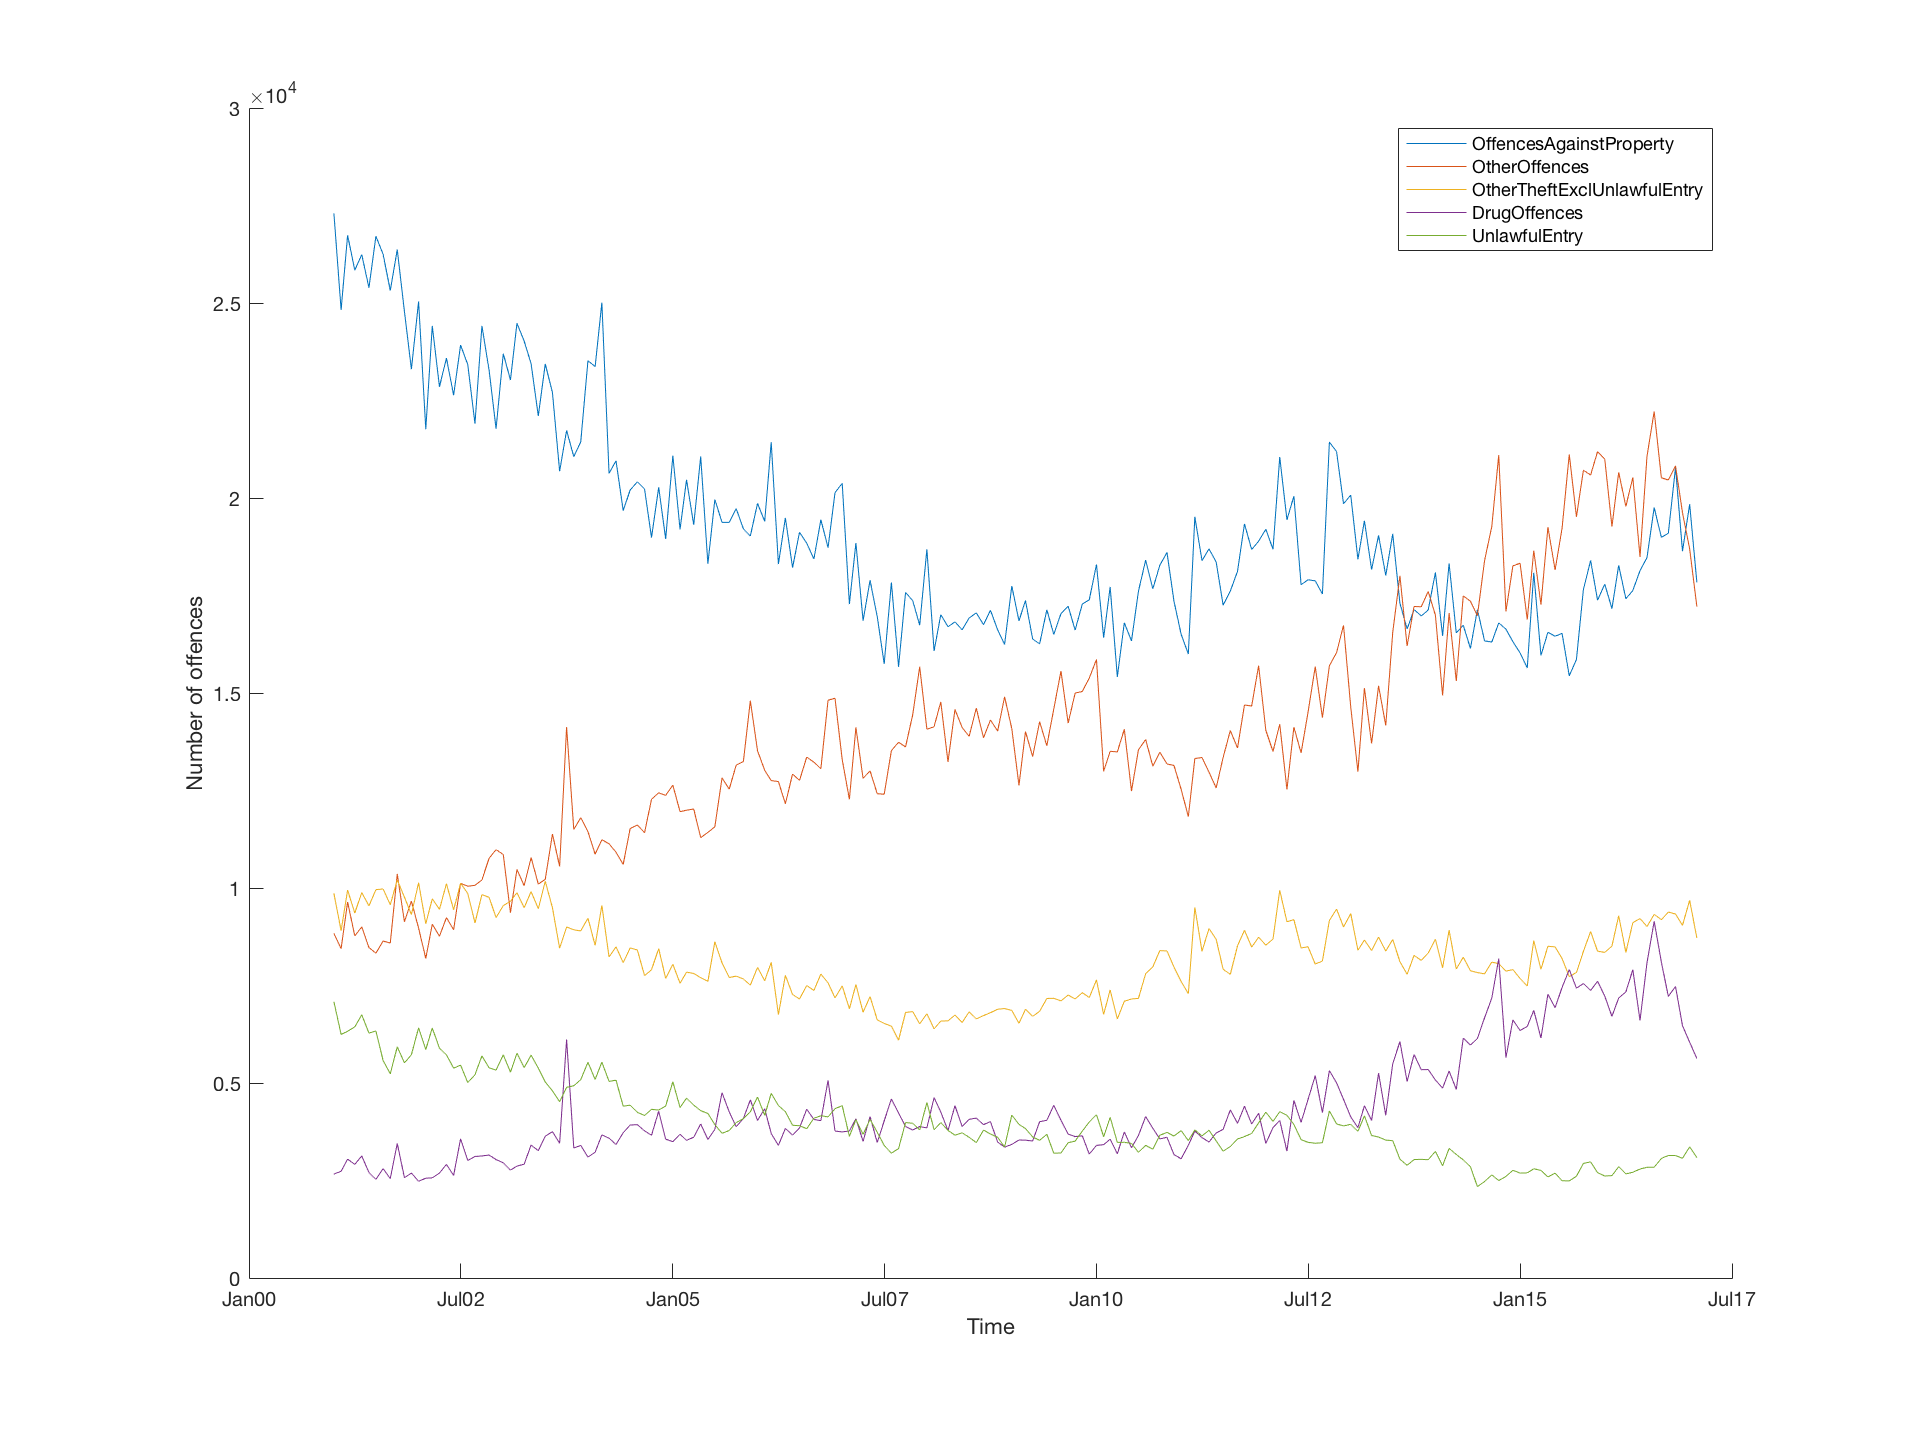
\includegraphics[width=\linewidth]{../images/top_offences_over_time}
\end{figure}

\section{Limitations}

\section{Conclusions}

\section{References}

\bibliographystyle{abbrvurl}
\bibliography{bibliography}

\end{document}
